\documentclass[10pt]{amsart}
\usepackage{amsmath,mathrsfs,graphicx}
%\usepackage{times}
\textwidth 4.5in  \textheight 7.125in
\newtheorem{theorem}{Theorem}
\newtheorem{remark}[theorem]{Remark}
\newtheorem{lemma}[theorem]{Lemma}
\newtheorem{proposition}[theorem]{Proposition}
\newtheorem{corollary}[theorem]{Corollary}
\newcommand{\comment}[1]{}
\begin{document}
\title{A note on  Costas arrays and cyclotomic permutations}
\author{Jordan Bell}
\email{jordan.bell@gmail.com}
\author{Qiang Wang}
\email{wang@math.carleton.ca}
\address{School of Mathematics and Statistics, Carleton
University, Ottawa, Ontario, Canada}
\thanks{This research was supported by an NSERC grant.}
\keywords{Costas arrays, singly periodic Costas arrays, primitive elements, cyclotomic
permutations, cyclotomy} \subjclass[2000]{Primary: 05B30;
Secondary: 05B15, 94A12, 11T22}


\begin{abstract}
In this paper we first  show that for all $q>7$, there does not
exist a primitive element $\alpha$ in $\mathbb{F}_q$ such that
$\alpha+\alpha^{-1}=1$. This answers a question of O. Moreno about a
certain construction for Costas arrays.  Then, the construction of
Costas arrays by cyclotomic permutations is considered. Necessary
conditions are given for a cyclotomic permutation to form a circular Costas
array. Further necessary conditions are proved on the index of a
cyclotomic permutation for it to form a circular Costas array. Finally,
research problems for Costas arrays are outlined.
\end{abstract}

\maketitle

\section{Introduction}
\label{section:introduction} An $m \times m$ {\em Costas array} is
an $m \times m$ permutation matrix (that is, a square matrix with
precisely one 1 in each row and column and all other entries 0)
for which all the vectors joining the pairs of 1's are distinct.
It is clear that a bijection $f:\{1,\ldots,m\} \to \{1,\ldots,m\}$, from
the columns to the rows (i.e. to each column $x$ we assign one and
only one row $f(x)$), gives a Costas array if and only if for $x
\neq y$ and $k \neq 0$ such that $1 \leq x, y, x+k, y+k \leq m$, we have
that
$f(x+k)-f(x) \neq f(y+k)-f(y)$.

Let $\pi:\mathbb{Z} \to \{1,\ldots,m\}$ be 
defined by $\pi(x)=y$ if $x \equiv y \pmod {m}$.
A bijection $f:\{1,\ldots,m\} \to \{1,\ldots,m\}$ is a {\em circular
Costas array} if for
$\pi(x) \neq \pi(y)$ and $\pi(k) \neq m$
we have that
$f(\pi(x+k))-f(\pi(x)) \not \equiv
f(\pi(y+k))-f(\pi(y)) \pmod{m+1}$.
Circular Costas arrays are a special
case of {\em singly periodic Costas arrays}, which are
bijections $f:\{1,\ldots,m\} \to \{1,\ldots,m\}$ such that
for $\pi(x) \neq \pi(y)$ and $\pi(k) \neq m$
we have that
$f(\pi(x+k))-f(\pi(x)) \neq
f(\pi(y+k))-f(\pi(y))$; an $m \times m$ singly periodic Costas
array is an $m \times m$ Costas array such that when it is repeated
horizontally on an $m \times \infty$ array, any $m \times m$
window is a Costas array.

Figure \ref{figure:6x6circular} shows a $6 \times 6$ circular Costas array
and Figure \ref{figure:6x6} shows a $6\times 6$ Costas array that fails to be
a circular Costas array. Indeed, for $x=5, y=1$, and $k=1$, we have
$f(\pi(x+k))-f(\pi(x))=f(6)-f(5)=-3$ and $f(\pi(y+k))-f(\pi(y))
=f(2)-f(1)=6-2=4$, and $-3 \equiv 4 \pmod{7}$.

\begin{figure}
\caption{$6\times 6$ circular Costas array. $f(1)=3,f(2)=2,f(3)=6,f(4)=4,
f(5)=5,f(6)=1$}
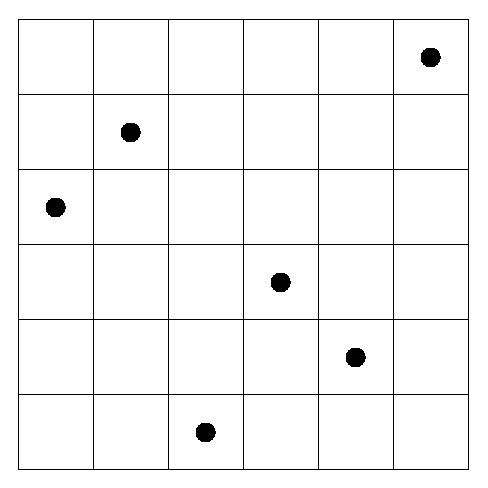
\includegraphics[scale=0.75,angle=-90]{6x6circular}
\label{figure:6x6circular}
\end{figure}

\begin{figure}
\caption{$6 \times 6$ Costas array that fails to be a circular Costas array.
$f(1)=2,f(2)=6,f(3)=5,f(4)=3,f(5)=4,f(6)=1$}
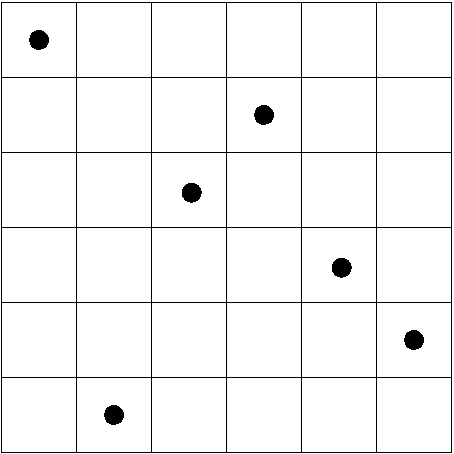
\includegraphics[scale=0.75,angle=-90]{6x6}
\label{figure:6x6}
\end{figure}

Let $c_m$ denote the number of $m \times
m$ Costas arrays and $c_m'$ denote the number of $m \times m$
circular Costas arrays. Trivially, $c_m' \leq c_m$ for all $m$.


Costas arrays were first considered by Costas \cite{costas1975} as
permutation matrices with ambiguity functions taking only the
values 0 and 1, applied to the processing of radar and
sonar signals. The use of Costas arrays in radar is summarized in
\cite[\S 5.2]{levanon}. % and \cite[\S 6.5]{skolnik}.
Costas arrays are also used in the design of optical orthogonal
codes for code division multiple access (CDMA) networks
\cite{maric1995}, and in the construction of low-density
parity-check (LDPC) codes \cite{chae2004}. Singly periodic Costas
arrays have applications to other combinatorial designs such as
Tuscan squares \cite{MR992291} and Vatican squares
\cite{MR1992965}, and in the design of sequences for
ultra-wideband impulse radio \cite{chu2004}, and circular Costas
arrays are related to a particular construction of Tuscan squares
\cite{periodicity} and are used in delay-Doppler imaging
\cite{MR1665811}. However, despite the many applications of Costas
arrays, there has been little theoretical work done on them for
more than 15 years, in particular no new constructions and no new
results on those $m$ for which Costas arrays of order $m$ exist.

Let us briefly recall some  known constructions and questions on
Costas arrays.  One can find more details in the survey papers
of Golomb and Taylor \cite{MR674209,golomb1984} and Drakakis \cite{drakakis}.
In the following, $p$ is taken to be a prime and $q$ a prime power.
 The known general
constructions for $m \times m$ Costas arrays are the Welch
construction for $m=p-1$ and $m=p-2$, the Lempel construction for
$m=q-2$, and the Golomb construction for $m=q-2$, $m=q-3$. Moreover,
if $q=2^k$, $k\geq 3$, the Golomb construction works for
$m=q-4$.
 The validity of the Welch and Lempel constructions is proved by
Golomb in \cite{MR749508}. The Golomb constructions for $m=q-3$ and
$m=2^k-4$ depend on the existence of (not necessarily distinct)
primitive elements $\alpha$ and $\beta$ in $\mathbb{F}_q$ such that
$\alpha+\beta=1$; the existence of such elements is proved by Moreno
and Sotero \cite{moreno1990} (Cohen and Mullen \cite{MR1209243}
give a proof with
less computational checking). Variants of the
above constructions include the Taylor variant of the Lempel
construction for $m=q-4$ when there is a primitive element $\alpha$
in $\mathbb{F}_q$ such that $\alpha^2+\alpha=1$ (Golomb 
\cite{golomb1992} proves that $q$ must be either 4, 5 or 9, or a prime $p
\equiv \pm 1 \pmod{10}$), Taylor variants of the Golomb construction
for $m=q-1$ when $q \neq 2^k$ and certain corner conditions are
satisfied and for $m=q$ when $q \equiv -1 \pmod{6}$ and certain
corner conditions are satisfied, and a few other variants which
yield Costas arrays of orders that are already covered above.
The total number of
$m \times m$ Costas arrays have
been enumerated for $m$ from 1 to 26 \cite{beard}.
It is known (cf. Drakakis \cite{drakakis}) that for all sufficiently large
$m$,
\[
c_m \leq
m!\bigg(\frac{40(m-1)}{m(m-2)}+\frac{9m^2-45m+60}{(m-3)(m-4)(m-5)}\bigg),
\]
and so $c_m=O((m-1)!)$.
Silverman,
Vickers and Mooney \cite{silverman} give probabilistic
estimates on the number of Costas arrays.
It is a very
interesting question to find more construction methods and to get
some information on the numbers of Costas arrays.

As we noted, circular Costas arrays are related to certain Tuscan
arrays. Golomb and Moreno \cite{periodicity} proved  that an $m
\times m$ circular Costas array exists if and only if $m+1$ is
prime, and conjectured that all circular Costas arrays are given
by the Welch construction.

In this paper we
first solve a problem of Moreno \cite[Question~2]{MR1992966} on the
existence of certain primitive elements in finite fields.
Then we propose studying Costas
arrays by using cyclotomic permutations  and obtain some necessary
conditions on the indices of cyclotomic permutations that define
circular Costas arrays.

\section{Results}
For a prime power $q$, let $\mathbb{F}_q$ be the finite field with
$q$ elements.
Let us first consider Moreno's question \cite[Question~2]{MR1992966} on
when there exists a
primitive element $\alpha$ in a finite field $\mathbb{F}_q$ such
that $\alpha+\alpha^{-1}=1$. We will show that such an $\alpha \in \mathbb{F}_q$
does not  exist for $q \neq 3, 4, 7$ and
thus it will not provide a new construction for $m \times m$ Costas arrays for
$m$ other than $4$ and $5$.  First of all it is easy to verify the
existence of a primitive element $\alpha$ such that $\alpha +
\alpha^{-1} =1$ in $\mathbb{F}_3$,  $\mathbb{F}_4$ and
$\mathbb{F}_7$. Indeed, $2$ is such a primitive element in
$\mathbb{F}_3$, a root of $x^2+x+1$ is such an element in
$\mathbb{F}_4=\mathbb{F}_2[x]/(x^2+x+1)$, and $3$ is such
an element in $\mathbb{F}_7$. For $q=2$, 1 is the only
primitive element in $\mathbb{F}_2$. Since $1+1=0 \neq 1$, there
exists no such $\alpha \in \mathbb{F}_2$.
For $q=5$, the primitive elements in $\mathbb{F}_5$ are 2 and
$3=2^{-1}$. But $2+2^{-1}=0=3+3^{-1}$, so no such $\alpha$ exists.
We now prove that for all other $q$, there exists no such $\alpha \in
\mathbb{F}_q$.

\begin{theorem}
For all prime powers $q>7$, there does not exist a primitive element
$\alpha \in \mathbb{F}_q$ such that $\alpha+\alpha^{-1}=1$.
\end{theorem}
\begin{proof}
Suppose there were a primitive element $\alpha \in \mathbb{F}_q$ such that
$\alpha+\alpha^{-1}=1$. Thus $\alpha^2+1=\alpha$. But
then $\alpha^3+\alpha=\alpha^2$, so $\alpha^3+\alpha^2+1=\alpha^2$ and
thus $\alpha^3=-1$. Therefore $\alpha^6=1$, which is a contradiction
for $q>7$. Hence if $q>7$, then
there does not exist a primitive element $\alpha \in \mathbb{F}_q$ such that
$\alpha+\alpha^{-1}=1$.
\end{proof}

We now study Costas arrays in terms of cyclotomic permutations of
finite fields.
Let $p$ be a prime. 
We take positive integers $n$ and $s$ such that
$ns=p-1$. Let $\alpha$ be a primitive element in $\mathbb{F}_p$.
We define
\[
C_0=\big \{\alpha^{jn}:j=0,\ldots,s-1 \big \},
\]
which is the subgroup
of $n$ powers of the
multiplicative group $\mathbb{F}_p^*=\mathbb{F}_p \setminus \{0\}$.
We define the {\em
cyclotomic cosets} as
\[
C_i(\alpha)=\alpha^i C_0, \quad i=0,\ldots,n-1.
\]
We remark that $C_0$ does not depend on the choice of 
primitive element $\alpha \in \mathbb{F}_p$ but that the cosets
$C_i(\alpha)$ do indeed depend on the choice of $\alpha$.

For $a_0,\ldots,a_{n-1} \in \mathbb{F}_p$, we define a {\em
cyclotomic mapping $f_{\alpha;a_0,\ldots,a_{n-1}}$ of index $n$}
$\mathbb{F}_p \to \mathbb{F}_p$  by
\[
f_{\alpha;a_0,\ldots,a_{n-1}}(x) =
\begin{cases}
0, &\textrm{if } x = 0,\\
a_i x,&\textrm{if } x \in C_i(\alpha), \quad i=0,\ldots,n-1.
\end{cases}
\]

\begin{lemma}
Let $\alpha,\beta$ be primitive elements in $\mathbb{F}_p$ and let
$f: \mathbb{F}_p \to \mathbb{F}_p$.
If there are $a_0,\ldots,a_{n-1} \in \mathbb{F}_p$ such that
\[
f(x)=\begin{cases}
0,&\textrm{if } x=0,\\
a_i x,&\textrm{if } x \in C_i(\alpha),\quad i=0,\ldots,n-1
\end{cases}
\]
then there are $b_0,\ldots,b_{n-1} \in \mathbb{F}_p$ such that
\[
f(x)=\begin{cases}
0,&\textrm{if } x=0,\\
b_i x,&\textrm{if } x \in C_i(\beta),\quad i=0,\ldots,n-1.
\end{cases}
\]
\end{lemma}
\begin{proof}
For some $k$, $\alpha=\beta^k$.
If $\gcd(k,n)=l>1$, let $k=lk_0$.
Then $\alpha^{(p-1)/l}=\beta^{k_0(p-1)}=1$, contradicting that
$\alpha \in \mathbb{F}_p$ is primitive. Therefore $\gcd(k,n)=1$.

Define $\psi:\{0,\ldots,n-1\} \to
\{0,\ldots,n-1\}$ by: $\psi(i)$ is the remainder of $ki$ after division by $n$.
Because $\gcd(k,n)=1$, $\psi$ is a bijection.
Let $b_0,\ldots,b_{n-1}$ be defined by $b_i=a_{\psi^{-1}(i)}$.

If $x \in C_i(\beta)$ then $x \in C_{\psi^{-1}(i)}(\alpha)$ and hence
$f(x)=a_{\psi^{-1}(i)}x=b_i x$.
\end{proof}

Thus the index of a cyclotomic mapping does not depend on the primitive element
used to define the cyclotomic cosets.

A {\em cyclotomic permutation of index $n$} is defined to be a
cyclotomic mapping of index $n$ that is a bijection $\mathbb{F}_p \to
\mathbb{F}_p$.
In
$\mathbb{F}_p^*$, $\log_\alpha(a_i)$ is defined to be the minimum
nonnegative integer $d$ such that $\alpha^d= a_i$.
The following remark is then clear.

\begin{remark}
\label{complete}
A cyclotomic mapping $f_{\alpha;a_0,\ldots,a_{n-1}}$ of $\mathbb{F}_p$
is a cyclotomic permutation of $\mathbb{F}_p$ if and only if
$\{\log_{\alpha}(a_i) + i \}$ is a complete residue system modulo
$n$.
\end{remark}


Certainly, any bijection $\mathbb{F}_p \to \mathbb{F}_p$ which
fixes 0 can be represented as a cyclotomic permutation of index at most
$p-1$  (cf. Niederreiter and Winterhof
\cite{MR2143454}). Indeed, let $f:\mathbb{F}_p \to \mathbb{F}_p$ be a
bijection
that
fixes 0 and let $\alpha$ be a primitive element in $\mathbb{F}_p$. Then the
cyclotomic cosets of index $p-1$
are given by $C_i(\alpha)=\{\alpha^i\}$ for $0 \leq i
\leq p-1$. Let $a_i=f(\alpha^i)\alpha^{-i}$. Then $f$ is a
cyclotomic permutation of index $p-1$. It is also clear that any
permutation of $\{1,\ldots,p-1\}$ can naturally be considered as
a permutation of $\mathbb{F}_p$ that fixes 0. Thus it is natural
to consider constructing $(p-1) \times (p-1)$ Costas arrays, for
$p$ prime, by cyclotomic permutations of $\mathbb{F}_p$.

For example, for $p=7$, the permutations $f$ and $g$ defined by $f(1)=6, f(2)=2, f(3)=1, f(4)=4,
f(5)=5, f(6)=3$ and $g(1)=3,g(2)=6,g(3)=1,g(4)=5,g(5)=4,g(6)=2$ define
$6 \times 6$ Costas arrays \cite{MR749508}. 3 is a primitive
element in $\mathbb{F}_7$. The divisors of $p-1=6$ are 1,2,3,6. Clearly $f$ is not a cyclotomic
permutation of index 1. If $f$ were a cyclotomic permutation of index 2, then
putting $C_0=\{2,4,1\}$ and $C_1(3)=\{6,5,3\}$, for some $a_0,a_1$ we would have
$f(x)=a_0x$ for $x \in
C_0$
and $f(x)=a_1x$ for $x \in C_1(3)$.
But $f(1)=6$, so $a_0=6$, which contradicts
$f(2)=2$. We can show in a similar way that $f$ is not a cyclotomic
permutation of index 3, and thus that $f$ is a cyclotomic permutation of least
index 6. On the other hand, for $a_0=3,a_1=5$, we find that $g$ is a cyclotomic
permutation of index 2.

Using the definitions of cyclotomic permutation and Costas array, we
can easily deduce the following necessary condition for
$f_{\alpha;a_0,\ldots,a_{n-1}}$ to give a $(p-1)\times (p-1)$ circular Costas
array.

\begin{proposition}
Let $f_{\alpha;a_0,\ldots,a_{n-1}}$ be a cyclotomic permutation of
$\mathbb{F}_p$. For $f$ to form a $(p-1) \times (p-1)$ circular Costas array,
it is necessary that for all $x\in C_i(\alpha)$, $y\in C_j(\alpha)$, $x\neq y$
such that $a_i = a_j$, that if $x+k \in
C_l(\alpha)$ and $y+k \in C_m(\alpha)$, $k\neq 0$, then $a_l \neq a_i$ or $a_m \neq a_i$.
\end{proposition}


 This is certainly not a sufficient condition, since for
example $f_{2;1,4,5,2,3}$ is a cyclotomic permutation of
$\mathbb{F}_{11}$, of index 5, that satisfies this condition but
which does not form a Costas array. It is worthwhile to
characterize when cyclotomic permutations produce Costas arrays.

In order to study possible indices of cyclotomic permutations of
$\mathbb{F}_p$ that can generate a $(p-1)\times(p-1)$ circular Costas array,
we shall employ the following result.


\begin{lemma}
\label{lemma:happen}
If there are distinct $x,y$ in some cyclotomic
coset $C_i(\alpha)$ such that $x+k$ and
$y+k$ are also in $C_i(\alpha)$, then this will happen in $C_0$.
\end{lemma}
\begin{proof}
By assumption, for some
distinct $x,y \in C_i(\alpha)$, it holds that $x+k,y+k \in C_i(\alpha)$ for
some fixed $k$.
Now, take $z=x\alpha^{-i}$, $w=y\alpha^{-i}$ and $l=k\alpha^{-i}$.
Clearly $z,w \in C_0$. Moreover,
\begin{eqnarray*}
z+l&=&x\alpha^{-i}+k\alpha^{-i}\\
&=&\alpha^{-i}(x+k),
\end{eqnarray*}
and since $x+k \in C_i(\alpha)$, we have that
$z+l=\alpha^{-i}(x+k) \in C_0$. Similarly,
$w+l \in C_0$, proving the claim.
\end{proof}

In the following two theorems we prove that cyclotomic
permutations of $\mathbb{F}_p$ of certain indices do not form
$(p-1) \times (p-1)$ circular Costas arrays (ignoring the fixed
point 0). We do this by showing that for these indices, there are
always two distinct pairs of elements in the cyclotomic coset
$C_0$ with equal differences. Indeed, Lemma \ref{lemma:happen}
says that if we can ever find such pairs of elements in a
cyclotomic coset, we will find them in $C_0$.

\begin{theorem} \label{evens}
For $ns=p-1$, if $s=2r \geq 4$
then there does not exist a cyclotomic permutation
of index $n$ that forms a circular Costas array.
\end{theorem}
\begin{proof}
We note that
\[
C_0=\big \{1,\alpha^n,\ldots,\alpha^{rn},
\alpha^{(r+1)n},\ldots,
\alpha^{(s-1)n} \big \}.
\]
Let $x=1$ and $y=\alpha^{(r+1)n}=-\alpha^n$; these are distinct
elements in $C_0$. But for $k=\alpha^n-1 \neq 0$ we obtain
\[
\begin{split}
&f_{\alpha;a_0,\ldots,a_{n-1}}(x+k)-f_{\alpha;a_0,\ldots,a_{n-1}}(x)\\
=&a_0(\alpha^n)-a_0(1)\\
=&a_0(\alpha^n-1),
\end{split}
\]
and
\[
\begin{split}
&f_{\alpha;a_0,\ldots,a_{n-1}}(y+k)-f_{\alpha;a_0,\ldots,a_{n-1}}(y)\\
=&f_{\alpha;a_0,\ldots,a_{n-1}}(-1)-f_{\alpha;a_0,\ldots,a_{n-1}}(-\alpha^n)\\
=&a_0(-1)-a_0(-\alpha^n)\\
=&a_0(\alpha^n-1),
\end{split}
\]
giving
\[
f_{\alpha;a_0,\ldots,a_{n-1}}(x+k)-f_{\alpha;a_0,\ldots,a_{n-1}}(x)=
f_{\alpha;a_0,\ldots,a_{n-1}}(y+k)-f_{\alpha;a_0,\ldots,a_{n-1}}(y)
\]
 for $x \neq y$ and $k \neq 0$.
Hence $f_{\alpha;a_0,\ldots,a_{n-1}}$ does not form a circular Costas array.
Thus, no cyclotomic permutation of index $n$ such that
$\frac{p-1}{n}=2r \geq 4$ forms a circular Costas array.
\end{proof}

\begin{theorem} \label{largep}
For $ns=p-1$, if $p>n^2+n+1$ then there does not exist a
cyclotomic permutation of index $n$ that forms a circular Costas array.
\end{theorem}
\begin{proof}
If there are distinct $x,y$ in $C_0$ such that
$x+k,y+k$ are in $C_0$ for some $k \not \equiv 0 \pmod{p-1}$, then
for any cyclotomic permutation $f_{\alpha;a_0,\ldots,a_{n-1}}$ of index $n$,
$f_{\alpha;a_0,\ldots,a_{n-1}}(x+k)-f_{\alpha;a_0,\ldots,a_{n-1}}(x)=
f_{\alpha;a_0,\ldots,a_{n-1}}(y+k)-f_{\alpha;a_0,\ldots,a_{n-1}}(y)$,
and thus does not form
a Costas array.
We shall prove that for all $n$ such that $p>n^2+n+1$ there exist
such $x,y,x+k,y+k$ in $C_0$.

There are $\frac{p-1}{n}$ $n$th powers in $\mathbb{F}_p^*$. Let
$\xi_1,\ldots,\xi_{\frac{p-1}{n}}$ be the $n$th powers in
$\mathbb{F}_p^*$. Consider all
$\frac{p-1}{n}\big(\frac{p-1}{n} - 1\big)$ differences $\xi_i -\xi_j$
between the pairs of $n$th powers $\xi_i, \xi_j$ with
$i\neq j$. If $\frac{p-1}{n}\big(\frac{p-1}{n} - 1\big)
>p-1$, then by the pigeonhole principle there exist $i_1, j_1, i_2,
j_2$ such that $i_1 \neq j_1$, $i_2 \neq j_2$
and $\xi_{i_1} -\xi_{j_1} = \xi_{i_2} -\xi_{j_2}$ in $\mathbb{F}_p$.
Solving $\frac{p-1}{n}\big(\frac{p-1}{n} -1\big)
> (p-1)$,
we have $p > n^2 + n +1$.
Let
$x=\xi_{i_1}$, $y =\xi_{i_2}$, and $k=\xi_{j_1} -\xi_{i_1}$.
\end{proof}

Using Theorem \ref{evens} and Theorem \ref{largep}, we obtain the
following.

\begin{corollary}
Let $p$ be an odd prime. Any $(p-1)\times
(p-1)$ circular Costas array is necessarily generated by a cyclotomic permutation of
$\mathbb{F}_p$ with least index $n>\sqrt{p}-1$. Moreover, if
$\frac{p-1}{n}$ is even (for example, if $n$ is odd), then it is
necessary that $n=\frac{p-1}{2}$.
\end{corollary}
\begin{proof}
By Theorem \ref{largep} it must be that $n^2+n+1 \geq p$,
therefore $(n+1)^2 > p$, hence $n > \sqrt{p}-1$. If
$\frac{p-1}{n}$ is even and is greater than 2, this contradicts
Theorem \ref{evens}.
\end{proof}

Nieddereiter and Winterhof \cite{MR2143454} show that
the number $P_n$ of cyclotomic
permutations of $\mathbb{F}_p$ of least index $n$ is given by
\[
P_n=\sum_{d|n} \mu\Big(\frac{n}{d}\Big)\Big(\frac{p-1}{d}\Big)^d d!,
\]
for $\mu$ the M\"obius function. We have the following.

\begin{corollary}
Let $p$ be an odd prime and let $p-1=2^ab$ for $b$ odd. Then
\[
c_{p-1}' \leq P_{\frac{p-1}{2}} + \sum_{d|b \atop
\frac{\lfloor \sqrt{p}\rfloor }{2^a} \leq d} P_{2^a d}.
\]
\end{corollary}

\comment{
If $p \equiv 1 \pmod 4$, then
\[ c_{p-1} \leq  P_{\frac{p-1}{2}}
+\sum_{\substack{\lfloor \sqrt{p} \rfloor \leq 2n \leq
p-1\\2n|p-1}} P_{2n},
\] and if $p \equiv -1 \pmod 4$, then
\[ c_{p-1} \leq \sum_{\substack{\lfloor \sqrt{p} \rfloor \leq 2n \leq p-1\\2n|p-1}}  P_{2n}. \]
\end{corollary}}

There are 17 inequivalent (distinct under the group of symmetries
of the square) $6 \times 6$ Costas arrays \cite{golomb1984}. In
Table \ref{costas6} we give the cyclotomic permutations of
$\mathbb{F}_7$ of least index that form  these  Costas arrays, with the
primitive element 3 of $\mathbb{F}_7$.
We note that it can be shown (by checking each) that none of the
$6 \times 6$ Costas arrays are given by cyclotomic permutations of
index 3; by Theorem \ref{largep} none have index 1.

We observe that if $f$ is a Costas array, then
its clockwise rotation by 90 degrees is given by $x \mapsto f^{-1}(-x)$.
In the following proposition we show that a Costas array is given by a
cyclotomic
permutation of index $n$ if and only if its rotations and reflections are given
by cyclotomic permutations of index $n$.

\begin{proposition}
For a prime $p=ns$, a $(p-1) \times (p-1)$ Costas array is given by
a cyclotomic permutation of $\mathbb{F}_p$ with index $n$ if
and only its reflections and rotations have index $n$.
\end{proposition}
\begin{proof}
Let $\alpha \in \mathbb{F}_p$ be primitive.
Let $f_{\alpha;a_0,a_1,\ldots,a_{n-1}}$ and $g_{\alpha;b_0,b_1,\ldots,b_{n-1}}$ be
cyclotomic mappings
of $\mathbb{F}_p$ of
index $n$. Define
a cyclotomic mapping $h_{\alpha;c_0,c_1,\ldots,c_{n-1}}$ of index $n$
by $c_i=b_{\log_\alpha(a_i)+i}a_i$. It is not difficult to see that
$h(x)=g(f(x))$ for all $x$, hence the composition
of cyclotomic mappings of index $n$ is a cyclotomic mapping of index $n$.
Therefore if a Costas array is given by a cyclotomic permutation
$f$ of $\mathbb{F}_p$ of index $n$,
its reflections $x \mapsto -f(x), x \mapsto f(-x), x \mapsto -f(-x)$
are cyclotomic permutations of index $n$.

Let $f_{\alpha;a_0,a_1,\ldots,a_{n-1}}$ be a cyclotomic permutation of $\mathbb{F}_p$ of index $n$.
Then by Remark \ref{complete}, for each $j$ there is exactly one $i$ such
that $j=\log_\alpha(a_i)+i$. Let $b_j=a_i^{-1}$.
Then
it is clear that the cyclotomic mapping $g_{\alpha;b_0,b_1,\ldots,b_{n-1}}$
is the inverse of $f$. Hence the
inverse of a cyclotomic permutation of index $n$ is a cyclotomic permutation
of index $n$. Therefore if a Costas array is given by a cyclotomic
permutation
$f$ of $\mathbb{F}_p$ of index $n$,
its rotations $x \mapsto f^{-1}(-x), x \mapsto f^{-1}(-f^{-1}(-x)),
x \mapsto f^{-1}(-f^{-1}(-f^{-1}(-x)))$
are cyclotomic permutations of index $n$.
\end{proof}


\begin{table}
\caption{Cyclotomic permutations of least index which give $6 \times 6$
Costas arrays}
\label{costas6}
\begin{tabular}{l|l|l}
Costas array&cyclotomic permutation&least index\\
\hline
6,1,4,3,5,2&$f_{3; 6, 6,4,5,6,1}$&6\\
6,1,4,5,3,2&$f_{3; 6, 6,4,5,3,2}$&6\\
6,1,4,2,3,5&$f_{3; 6, 6,4,2,4,2}$&6\\
6,1,3,4,2,5&$f_{3; 6, 1,4,2,1,6}$&6\\
5,1,6,3,4,2&$f_{3; 5, 2,4,5,6,5}$&6\\
5,4,1,6,2,3&$f_{3; 5, 5,2,4,5,6}$&6\\
5,2,6,1,4,3&$f_{3; 5, 2,1,4,2,5}$&6\\
6,1,5,3,2,4&$f_{3; 6, 4,4,3,6,6}$&6\\
6,5,1,3,4,2&$f_{3; 6,5}$&2\\
6,2,1,4,5,3&$f_{3; 6, 5,1,4,1,1}$&6\\
6,2,1,5,3,4&$f_{3; 6, 5,1,3,3,2}$&6\\
5,3,6,1,2,4&$f_{3; 5, 2,5,3,2,6}$&6\\
5,2,6,1,3,4&$f_{3; 5, 2,1,3,2,2}$&6\\
5,3,2,6,1,4&$f_{3; 5,3}$&2\\
6,4,5,1,3,2&$f_{3; 6, 4,2,5,2,2}$&6\\
6,2,4,1,5,3&$f_{3; 6, 6,1,4,2,1}$&6\\
6,3,2,4,5,1&$f_{3; 6, 3,5,6,1,1}$&6
\end{tabular}
\end{table}

\section{Conclusions and research problems}
In this paper we  have answered a question of Moreno on the
existence of primitive elements $\alpha$ in $\mathbb{F}_q$ such
that $\alpha+\alpha^{-1}=1$. We have  proposed studying Costas
arrays, in particular circular Costas arrays, by using cyclotomic
permutations of finite fields. We have shown that for $p$ a prime
and $ns=p-1$, if $s=2r \geq 4$ or $p>n^2+n+1$ then there does
not exist a cyclotomic permutation of index $n$ that forms a
circular Costas array of size $(p-1)\times (p-1)$.
Hence it gives us a lower bound for the index of a
cyclotomic permutation of $\mathbb{F}_p$ which generates a
circular Costas array. We now outline several open problems on
Costas arrays.

As we remarked in Section \ref{section:introduction}, it is known
that for all $q$, there exist primitive elements $\alpha,\beta \in
\mathbb{F}_q$ such that $\alpha+\beta=1$
\cite{MR1209243,moreno1990}. Moreno \cite{MR1992966} asks for estimates
for how many such pairs of primitive elements exist.
We remark that if a prime $p$ is a
Mersenne exponent for which there exists a primitive trinomial
$t(x)=x^p+x^r+1$ over $\mathbb{F}_2$, then we can explicitly
obtain primitive elements $\alpha,\beta \in \mathbb{F}_{2^p}$ such
that $\alpha+\beta=1$. Indeed, let $\gamma \in \mathbb{F}_{2^p}$
be a root of $t(x)$. Then $t(\gamma)= \gamma^p+\gamma^r+1=0$ and
thus $\gamma^p+\gamma^r=1$. It is easy to see that
$\gcd(p,2^p-1)=1$ and $\gcd(r,2^p-1)=1$, and thus
$\alpha=\gamma^p$ and $\beta=\gamma^r$ are primitive elements in
$\mathbb{F}_{2^p}$ such that $\alpha+\beta=1$. For example, Brent,
Larvala and Zimmermann \cite{MR2114660} show that over
$\mathbb{F}_2$ the only primitive polynomials of degree $6972593$
(which is a Mersenne exponent) are
$t(x)=x^{6972593}+x^{3037958}+1$, and its reciprocal
$x^{6972593}+x^{6972593-3037958}+1$. Thus there is a primitive
element $\gamma \in \mathbb{F}_{2^{6972593}}$ such that
$t(\gamma)=0$, i.e. $\gamma^{6972593}+\gamma^{3037958}+1=0$. Since
$\gcd(2^{6972593}-1,6972593)=1$ and
$\gcd(2^{6972593}-1,3037958)=1$, $\alpha=\gamma^{6972593}$ and
$\beta=\gamma^{3037958}$ are both primitive elements in
$\mathbb{F}_{2^{6972593}}$, and
$\alpha+\beta=1$.



It is also very interesting to know whether there is a general
method of constructing Costas arrays  from cyclotomic permutations
of certain indices. Further study of cyclotomic
permutations might be helpful for handling 
the conjecture of Golomb and Moreno on circular Costas arrays
\cite{periodicity} and the conjecture of Golomb and Taylor on singly
periodic Costas arrays \cite{golomb1984}. In particular, estimates
on the number of circular Costas arrays are interesting because
proving $c_{p-1}' = 2(p-1)\phi(p-1)$ is equivalent to proving the
conjecture of Golomb and Moreno.

%As well, circular Costas arrays are in
%particular singly periodic Costas arrays,  and it could be useful
%to study singly periodic Costas arrays constructed using
%cyclotomic permutations.
% Golomb and Taylor \cite{golomb1984} conjectured that single periodicity characterizes the Welch
%construction.

Let $\mathbb{N}$ be the positive integers.
It is unknown whether for all
$m \in \mathbb{N}$ there exists a Costas array of order $m$, and indeed it is unknown
whether for all sufficiently large $m$ there exists a Costas array of order $m$.
It is natural to ask whether
there exist Costas arrays of order $m$ for all $m \in A$, for some subset
$A \subset \mathbb{N}$ of positive density. All the known constructions
for Costas arrays are for integers $m$ such that $|m-q| \leq 5$ for some
prime power
$q$. It is well known that the prime powers have density 0 in $\mathbb{N}$,
hence the set of all $m$ for which a Costas array is known to exist
has density 0 in $\mathbb{N}$.

It would be very desirable to find classes of permutation
polynomials  over finite fields which generate Costas arrays. This
problem was studied by Chu \cite{MR1992961}, who gave a simple
generalization of  the Welch, Lempel and Golomb constructions for
Costas arrays in terms of permutation polynomials.

\section*{Acknowledgements} We would like to thank the anonymous
referee for helpful suggestions.

\bibliographystyle{amsplain}
\bibliography{costas}

\end{document}
